\documentclass{article}
\usepackage{graphicx}

\title{
\textbf{pacman-racket} \\
\textit{User Guide}\\
A pragmatic implementation of Pacman in Racket\\
}

\author{
    Alessandro Zanzi,
    Filippo Piloni,\\
    Jeferson Morales Mariciano,
    Paolo Deidda
}
\date{
USI \\
Faculty of Informatics \\
[\baselineskip]  2021/2022
}


\begin{document}
%%%%%%%%%%%%%%%%%%%%%%%
%%%%%%%%%%%%%%%%%%%%%%%
%%%%%%%%%%%%%%%%%%%%%%%
\begin{titlepage}
\maketitle  
\thispagestyle{empty}
\end{titlepage}
%%%%%%%%%%%%%%%%%%%%%%%
%%%%%%%%%%%%%%%%%%%%%%%
%%%%%%%%%%%%%%%%%%%%%%%
\begin{abstract}
Conceptualization, research and thinking out-of-the-box
to implement the well-known classic game Pac-man
using the Racket functional programming language.\\
To develop this project, our group used abstractions and open-source tools to develop five files using Racket and linking them together to clarify the divisions between the various parts of the program and their respective functions.\\
To better organize this project, we used several instruments such as GitHub to be able to work at the program at any moment.\\
Using the knowledge developed during the lectures and the guides provided by Racket Documentation, the result of the project was a working revisited version of the game Pac-Man composed by one level where the ghosts move using a contrast logic that considers Pac-Man's position in the map.

\end{abstract}
\clearpage
\tableofcontents
\clearpage

\section{Guide}

\subsection{Game logic}
 The player must guide a yellow spherical creature, called Pac-Man, making it eat all the numerous dots scattered inside the maze and, in doing so, he must avoid being touched by four ghosts, or the game will be over. In order to make the game easier for the player, there are four "power pellets" in the corners of the screen that turn the situation by making Pac-Man able to touch ghosts without ending the game. Each dot taken will increase the score of 10 points, instead cherries and powerpellets are worth 100 points.

\subsection{UI}
\begin{center}
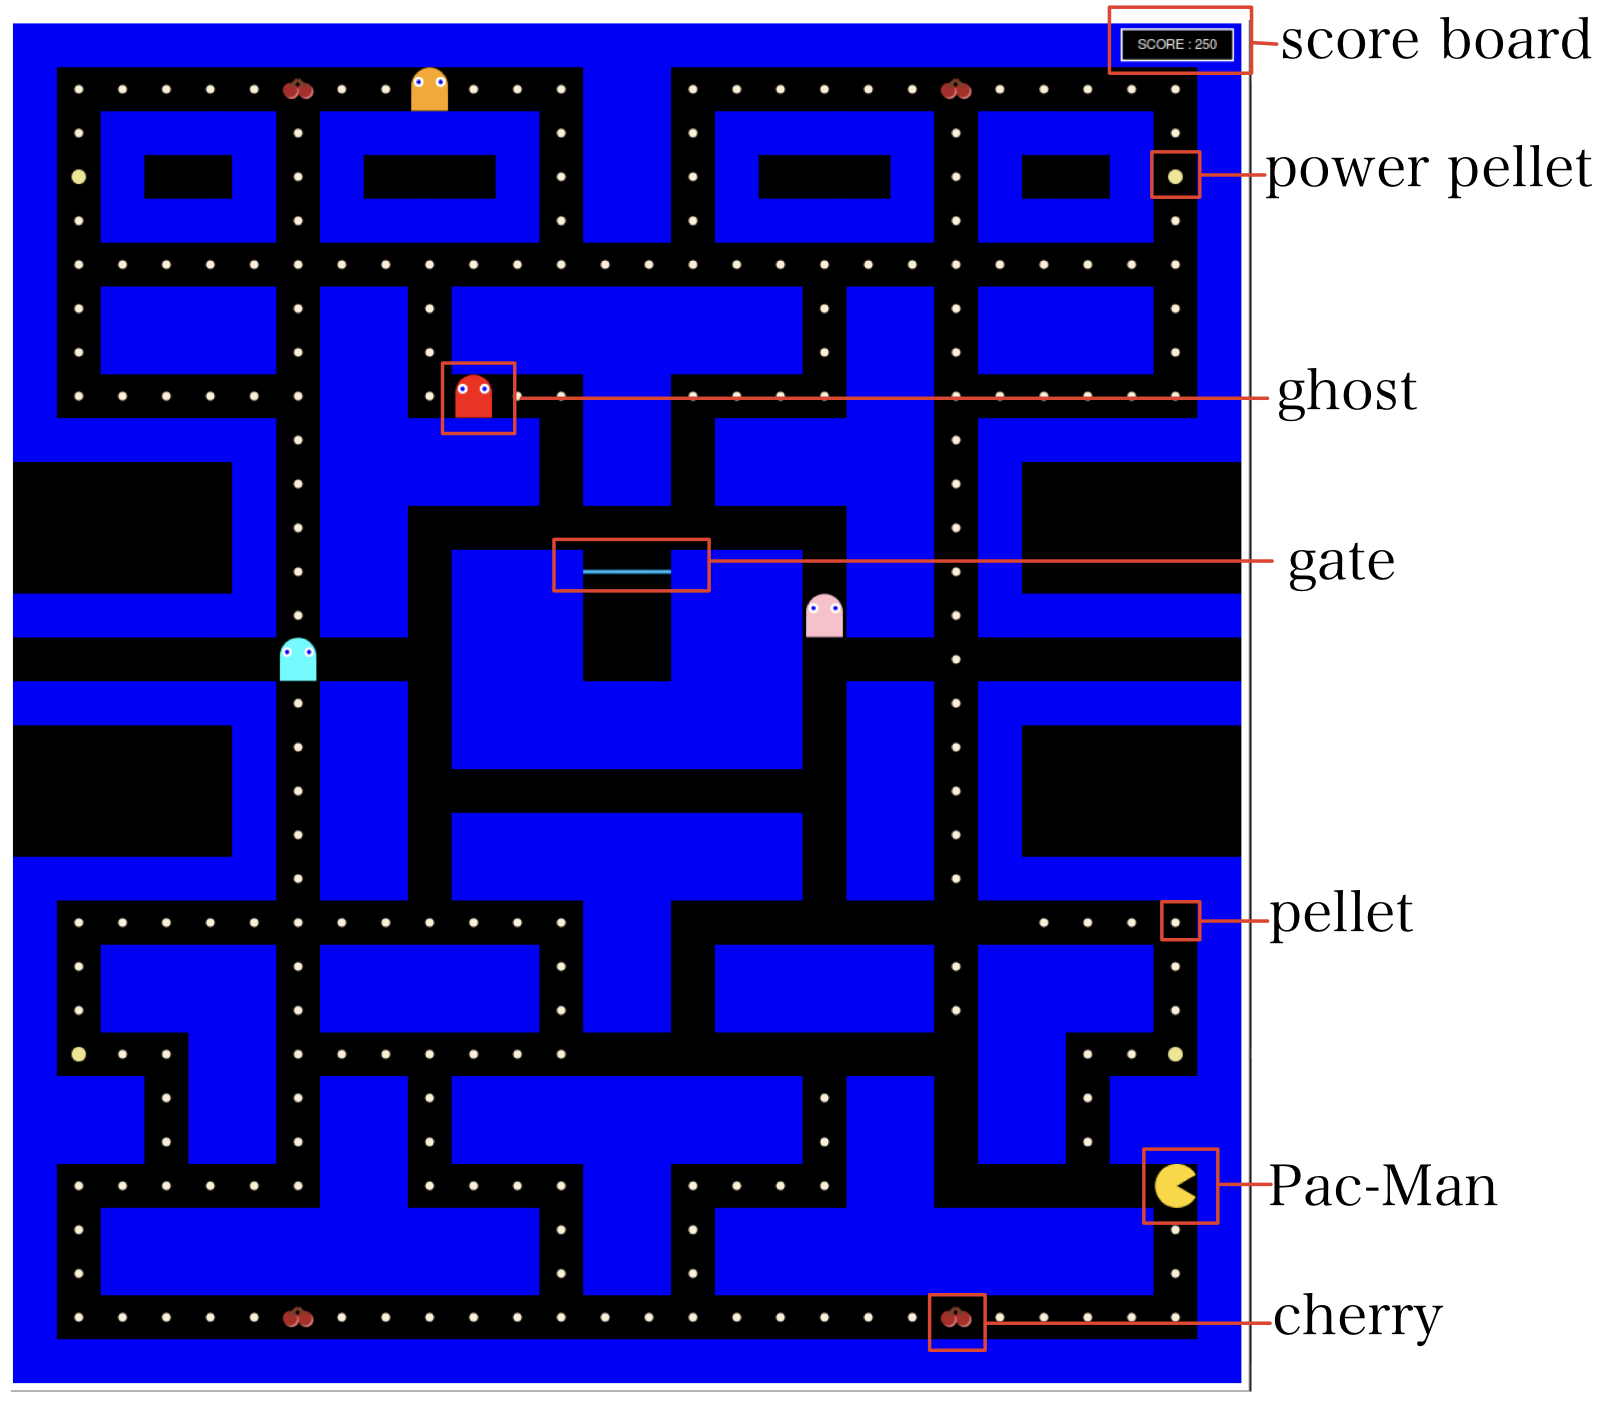
\includegraphics[width=12cm]{./images/user_interface.png}
\end{center}
The gaming window is completely occupied by the game screen (figure above), which is composed by the main area and the score display. While the score display keep track of the actual score, the main area is the most important part of the game. It is composed by several images that rapresents the part of the game, such as ghosts, pac-man, pellets and powerpellets.
 
\subsection{Key guide}
The player interact with Pac-Man with the four keys: \texttt{up}, \texttt{down}, \texttt{left} and \texttt{right}, to move in the respective direction.
\\
Is possible to press the key \texttt{Q} to end the game at any time.
 
\section{Usage}
  
\subsection{Setting}\label{setting}
To run the game the player needs the DrRacket IDE or raco, which is the Racket command line tool.\\
\\
To make the process easier the user can create an executable binary to have a clickable file which will start the game automatically when clicked. To create this file there are two ways:
\subsubsection{DrRacket executable}

The first require the drRacket compiler, once open upload the \textit{main.rkt}, click on \textit{Racket} above in the toolbar and finally click \textit{Create Executable...} in the drop-down menu. This will create a compressed folder (.tgz) in the selected directory which must be uncompressed. Once inside \textit{main/bin} folder there will be a file called \textit{main} ready to be clicked to start the game.

\subsubsection{raco executable}
For the second way is sufficient to open the terminal, go to the \textit{pacman-racket} folder and input the following terminal command:
\begin{center}
 \texttt{raco exe main.rkt}
\end{center}

This will create an executable binary in the \textit{pacman-racket} folder that will allow the user to start the game just by cliking on it.

\subsection{Start and Stop}
In order to start the game you have to open the \textit{main.rkt} file and press the \textit{run} button or press together the two keys \textit{ctrl} + \textit{R}.\\
If the executable file has been installed, to run the game will be sufficient to double click on it.\\
When a win or a loss occurs the player quits the game by closing the window. To play another round the player can run the program again as indicated in \ref{setting}.

 \end{document}
